The shape of the offering formula is always the same. It opens with the same standard phrase, invokes a god to pass along the offering, lists the offerings then names the recipient.

\section*{\indexed{Htp-di-nsw}}
\markboth{Outline}{Htp-di-nsw}
\addcontentsline{toc}{section}{Htp-di-nsw}

\begin{figure} [H]
	\centering
	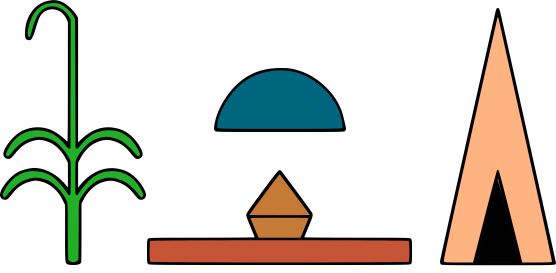
\includegraphics[width=0.4\textwidth]{../images/htp-di-nsw}
	\caption{Htp-di-nsw as commonly rendered in hieroglyphs}
\end{figure}

Many renditions of the offering formula begin with this compound expression. The exact interpretation is debated, but this is often rendered as "a royal offering" or "an offering given by the king".

This expression is sometimes used to describe an offering formula.

By convention the t from \indexed{nswt} is dropped, although it often appears in writing and inscriptions.

The order of the words when written is a case of \textit{\indexed{honorific transposition}}, with the \indexed{nswt} part written first. This is to show the importance of the king, and also applies to names of gods and the word nTr which loosely translates to "god".

\subsection*{Htp}

\begin{figure} [H]
	\centering
	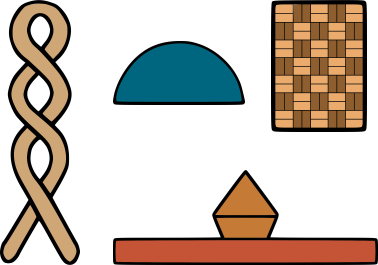
\includegraphics[width=0.275\textwidth]{../images/htp}
	\caption{A more complete spelling of \indexed{Htp} - \textbf{H t p} [Htp]}
\end{figure}

The word \indexed{Htp} has no precise translation into English, and is variously rendered as "contentment", "peace" or "offering". This is sufficient to grasp its true meaning, since offerings are intended to bring comfort and bliss.

\begin{figure} [H]
	\centering
	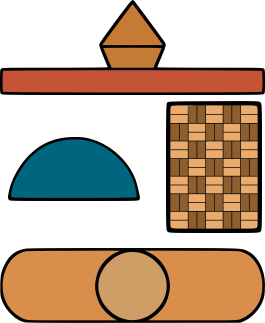
\includegraphics[width=0.175\textwidth]{../images/htp2}
	\caption{Another spelling of \indexed{Htp} - \textbf{Htp} t p [X4]}
\end{figure}

\subsection*{di}

\begin{figure} [H]
	\centering
	\includegraphics[width=0.125\textwidth]{../recoloured-tuxscribe-hieroglyphs/png/X8}
	\caption{the (r)di hieroglyph - X8}
\end{figure}

This word is a verb, (r)\indexed{di} - to give, which in older writings is sometimes rendered as \indexed{rdi} rather than di. It also appears later in the formula, but with a suffix pronoun, either .f, .s or .sn depending on the god(s) invoked.

\begin{figure} [H]
	\centering
	\includegraphics[width=0.375\textwidth]{../recoloured-tuxscribe-hieroglyphs/png/D37}
	\caption{the (r)di hieroglyph commonly used when writing di.f - D37}
\end{figure}

\subsection*{nswt}

The term nswt means the king or ruler. It was treated with great reverence as the embodiment of the institution of statehood, which was unique in its earliest form.

In older Egyptological works it is transliterated as swtn, but it is now believed that the order of the hieroglyphs is a form of \indexed{honorific transposition}.

\section*{prt-xrw}
\markboth{Outline}{prt-xrw}
\addcontentsline{toc}{section}{prt-xrw}

\begin{figure} [H]
	\centering
	\includegraphics[width=0.25\textwidth]{../recoloured-tuxscribe-hieroglyphs/png/O3}
	\caption{the prt-xrw hieroglyph - O3}
\end{figure}

The expression \indexed{prt-xrw} is usually translated as "\indexed{voice offering}", although it more directly means "emerging from voice".

The hieroglyph contains the bread and beer signs, but this is by convention, and doesn't necessarily mean that the voice offering includes bread and beer.

\section*{Offering(s)}
\markboth{Outline}{Offerings}
\addcontentsline{toc}{section}{Offerings}

\begin{figure} [H]
	\centering
	
\includegraphics[width=0.875\textwidth]{../images/xt-nb-nfr-wab-anxt-ntr-im}
	\caption{\textbf{x t nb}(t) \textbf{n f r} nfr \textbf{wab} \textbf{anx} n x \textbf{t nTr i m}}
\end{figure}

Thee is something of a standard list of offerings, which is usually terminated with the expression xt nbt nfrt wabt anxt nTr im - all the beautiful and pure things on which a god lives.

\subsection*{Bread - t}

\begin{figure} [H]
	\centering
	\includegraphics[width=0.2\textwidth]{../recoloured-tuxscribe-hieroglyphs/png/X1}
	\caption{the t hieroglyph - X1}
\end{figure}

Bread\index{bread} was a staple in the diet of Ancient Egypt, and bread making and consumption was deeply integrated into their culture.

It was primarily made from emmer \indexed{wheat} or \indexed{barley}, which was ground into \indexed{flour} using stones. The dough, made by mixing with \indexed{water}, and sometimes \indexed{honey} or \indexed{oil}, was left to naturally ferment, giving it a slightly sour flavour. Baking was usually done in conical \indexed{clay} \indexed{oven}s, where the dough was either placed on the oven walls, or baked in molds.

The hieroglyph for (r)di, X8, represents a sacrificial loaf, although it is a highly stylised rendition. The hieroglyph for t, X1, is also a stylised loaf. In the prt-xrw hieroglyph we can see X3 also used to represent a loaf.

\begin{figure} [H]
	\centering
	\includegraphics[width=0.125\textwidth]{../recoloured-tuxscribe-hieroglyphs/png/X3}
	\caption{the bread hieroglyph - X3}
\end{figure}

\subsection*{Beer - Hnqt}

Beer\index{beer} was an integral part of daily life in ancient Egypt, enjoyed by both the rich and the poor. Famously it was used to pay workers on the great royal projects, including the construction of the \indexed{Great Pyramid} of \sname{Giza}.

\begin{figure} [H]
	\centering
	\includegraphics[width=0.125\textwidth]{../recoloured-tuxscribe-hieroglyphs/png/W22}
	\caption{the Hnqt hieroglyph - W22}
\end{figure}

It was primarily made from the aforementioned \indexed{bread}, which was crumbled into \indexed{water} and left to ferment. The resulting brew was thick and nutritious, often flavoured with herbs, \indexed{honey}, or \indexed{fruit}s.

\subsection*{Oxen - kAw}

\begin{figure} [H]
	\centering
	\includegraphics[width=0.25\textwidth]{../recoloured-tuxscribe-hieroglyphs/png/F1}
	\caption{the kA(w) hieroglyph - F1}
\end{figure}

In ancient Egypt, \indexed{oxen}, castrated \indexed{bull}s, were highly valued for their critical role in agriculture and daily life. These sturdy animals were used for plowing fields, threshing grain, and transporting heavy loads, making them indispensable for farming communities along the Nile.

Bulls\index{bull} and \indexed{cow}s themselves were often part of religious ceremonies and offerings, representing strength and fertility. The \indexed{cow} was sacred to \nname{Hathor}, and certain sacred bulls were considered as gods themselves, including the \nname{Apis}, \nname{Mnevis} and \nname{Buchis} bulls.

Beef seems to have been considered somewhat of a luxury and was typically reserved for the elite and for special occasions.

Tomb paintings and carvings frequently depicted scenes of cattle being tended to, highlighting their importance in both practical and ceremonial contexts.

\subsection*{Fowl - Apdw}

\begin{figure} [H]
	\centering
	\includegraphics[width=0.2\textwidth]{../recoloured-tuxscribe-hieroglyphs/png/H1}
	\caption{the Apd(w) hieroglyph - H1}
\end{figure}

In ancient Egypt, \indexed{fowl} such as \indexed{duck}s, geese\index{goose}, pigeons, and quails played a significant role in both daily life and religious practices. In particular pigeons were trained as carriers for communication.

These birds were commonly raised in households and on farms, as well as being harvested from the river itself. They provided a source of meat, eggs, and feathers.

The Egyptians employed various techniques to catch wild birds, including netting and trapping. Fowl were often depicted in tomb paintings and reliefs, showcasing their importance in the Egyptian diet and culture.

\subsection*{Alabaster - Ss}

\begin{figure} [H]
	\centering
	\includegraphics[width=0.125\textwidth]{../recoloured-tuxscribe-hieroglyphs/png/V6}
	\caption{the Ss hieroglyph - V6}
\end{figure}

Alabaster, more specifically \indexed{calcite} \indexed{alabaster} or \indexed{travertine}, is a type of finely-grained translucent \indexed{stone}. It was highly prized in ancient Egypt for its beauty and versatility. This soft, workable material was especially favoured for sculpting intricate \indexed{statue}s, jars, and ceremonial vessels due to its smooth surface and ability to be carved with great precision. It was also employed in the production of \indexed{canopic jar}s that held the organs of the deceased during mummification.

\subsection*{Linen - mnxt}

\begin{figure} [H]
	\centering
	\includegraphics[width=0.25\textwidth]{../recoloured-tuxscribe-hieroglyphs/png/S27}
	\caption{the mnxt hieroglyph - S27}
\end{figure}

Linen.

It is fairly common to see alabaster and linen using a combined hieroglyph.

\begin{figure} [H]
	\centering
	\includegraphics[width=0.25\textwidth]{../recoloured-tuxscribe-hieroglyphs/png/S113}
	\caption{the Ss-mnxt hieroglyph - S113}
\end{figure}

\section*{God(s)}
\markboth{Outline}{God(s)}
\addcontentsline{toc}{section}{God(s)}

\subsection*{Anubis, who sits on his mountain}
\addcontentsline{toc}{subsection}{Anubis, who sits on his mountain}

\begin{figure} [H]
	\centering
	\includegraphics[width=0.0625\textwidth]{../recoloured-tuxscribe-hieroglyphs/png/C6}
	\hspace{0.03125\textwidth}
	\includegraphics[width=0.125\textwidth]{../recoloured-tuxscribe-hieroglyphs/png/E16}
	\includegraphics[width=0.125\textwidth]{../recoloured-tuxscribe-hieroglyphs/png/E17}
	\includegraphics[width=0.125\textwidth]{../recoloured-tuxscribe-hieroglyphs/png/E18}
	\caption{Single hieroglyphs for inpw - C6, E16, E17 and E18}
\end{figure}

Anubis is one of ancient Egypt's most revered and enigmatic deities. He is widely recognized as the god of mummification and the protector of the dead. He was often invoked in offering formulae, especially the oldest examples we have from the \indexed{Old Kingdom}.

\begin{figure} [H]
	\centering
	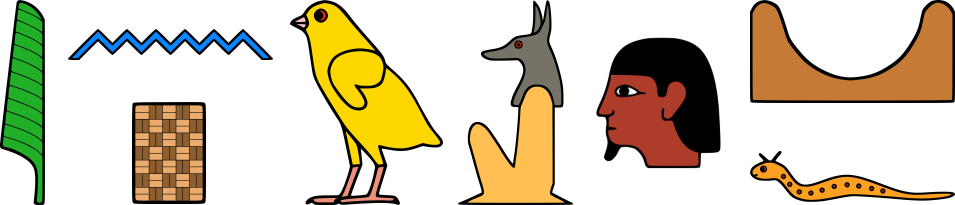
\includegraphics[width=0.875\textwidth]{../images/inpw-tpy-dwf}
	\caption{Anubis, who sits on his mountain\\\textbf{i n p w} [inpw] \textbf{tp} (y) \textbf{Dw.f}}
\end{figure}

Often depicted as a man with the head of a \indexed{jackal}, or entirely as a jackal, Anubis embodies the dual aspects of fear and reverence that surrounded death and the afterlife in ancient Egyptian culture.

\begin{figure} [H]
	\centering
	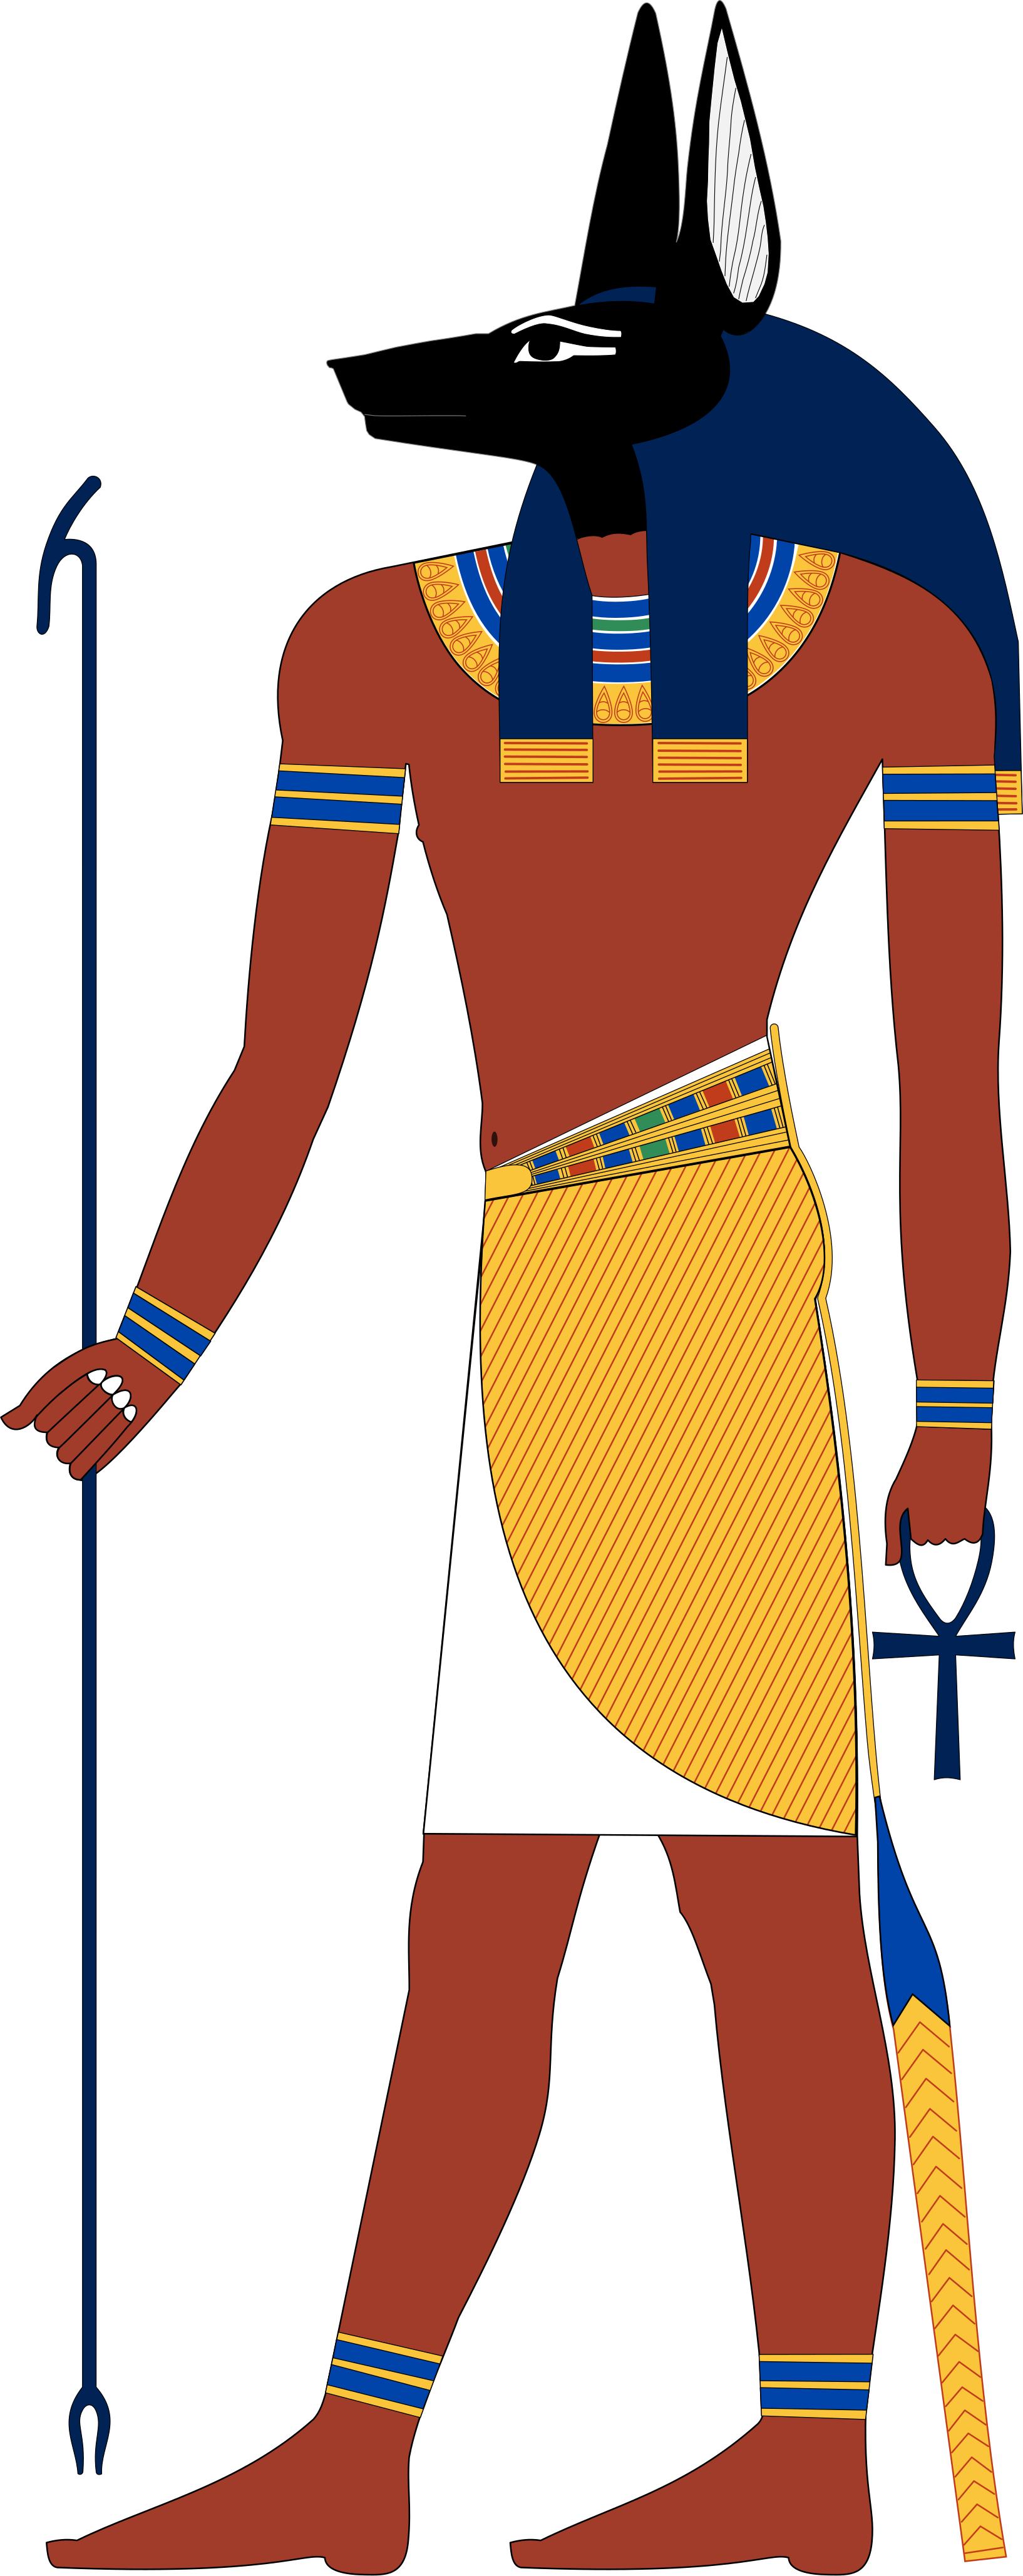
\includegraphics[width=0.5\textwidth]{../images/anubis}
	\caption{A standard depiction of Anubis}
\end{figure}

\subsubsection*{Origins and myths}
\addcontentsline{toc}{subsubsection}{Origins and myths}
The worship of \nname{Anubis} goes back to the predynastic period of Egyptian history.

His association with the \indexed{jackal} - a creature commonly seen around cemeteries and tombs - emphasize his role as a guardian of the necropolis, where the dead were laid to rest.

Initially, he was considered the foremost deity of the dead, a role later overshadowed by Osiris. However, \nname{Anubis} retained significant influence as the embalmer and guide of souls. Myths recount his critical role in the legend of \nname{Osiris} - he embalmed \nname{Osiris} after his murder by \nname{Seth}, making him the first \indexed{mummy} and setting the standards for \indexed{embalming} rites.

\subsubsection*{Iconography and symbols}
\addcontentsline{toc}{subsubsection}{Iconography and symbols}
The iconography of \nname{Anubis} is striking and distinctive. He is frequently depicted as a jackal, in a crouching or alert position, sometimes vigilant at the entrance of a tomb. His sleek black body has the colour associated with embalming, rebirth and the fertile soil of the Nile inundation.

\begin{figure} [H]
	\centering
	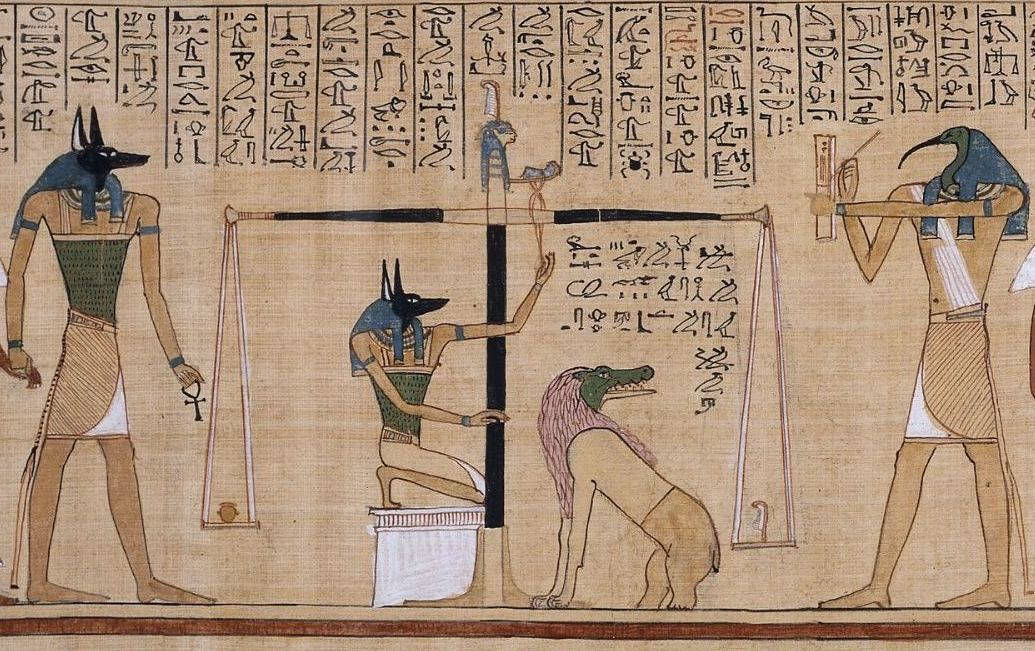
\includegraphics[width=0.75\textwidth]{../photos/Anubis_Hunefer}
	\caption{The weighing of the heart from the Book of the Dead of Hunefer}
\end{figure}

\nname{Anubis} was commonly depicted in the \indexed{weighing of the heart} ceremony - weighing the hearts of the deceased against the feather of \nname{Ma'at}, the goddess of truth and justice, in the Hall of two Ma'ats. This ceremony determined whether the deceased could continue in the journey to the afterlife.

\begin{figure} [H]
	\centering
	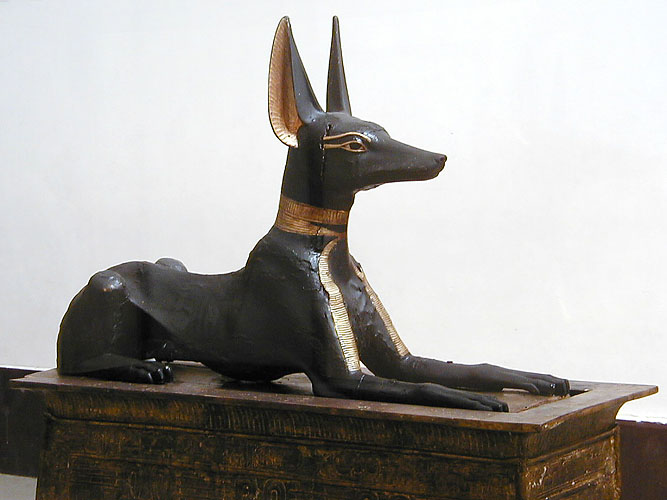
\includegraphics[width=0.75\textwidth]{../photos/Tutankhamun_Jackal}
	\caption{A guardian jackal statue from the tomb of Tutankhamun\\(Photo by Jon Bodsworth)}
\end{figure}

In another common representation, \nname{Anubis} is shown attending to a mummy, highlighting his role in embalming.

\begin{figure} [H]
	\centering
	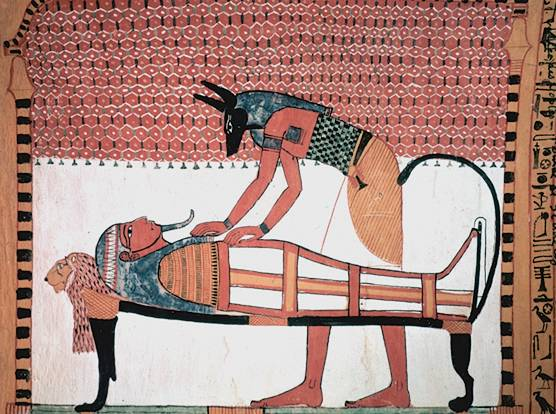
\includegraphics[width=0.75\textwidth]{../photos/Anubis_Sennedjem}
	\caption{Anubis, depicted attending the mummy of Sennedjem}
\end{figure}

His primary symbols include the \indexed{flail} reflecting his purifying role in selecting those deserving of the afterlife, and the \indexed{imy-wt}, or "\indexed{Anubis fetish}" - a stuffed, headless animal skin supported by a rod. In addition he is often depicted with the symbols of godhood, the \indexed{ankh}, a symbol of life and the \indexed{wAs} sceptre, signifying his authority.

\subsubsection*{Cult and worship}
\addcontentsline{toc}{subsubsection}{Cult and worship}
The worship of \nname{Anubis} was pervasive throughout Egypt, but there was a significant cult centre at sAkA, known by the \indexed{Greek}s as \sname{Cynopolis} (the "City of the Dog"). Priests of Anubis were tasked with overseeing mummification and funerary rites, donning jackal masks during ceremonies to invoke his presence. Rituals performed in his honour aimed to ensure the safe passage of the dead into the afterlife, with particular emphasis on purity and protection.

Amulets bearing the likeness of Anubis or his symbols were commonly placed among the burial goods, intended to ward off malevolent forces and guide the deceased through the treacherous journey to the afterlife. These artefacts, often inscribed with spells from the \indexed{Book of the Dead}, reflect strong belief in the ability of Anubis to safeguard and guide the deceased.

\subsubsection*{Legacy}
The legacy of Anubis endured well beyond the end of the pharaonic era. His image and role were integrated into Greco-Roman culture, where he was often syncretized with \nname{Hermes}, or forming the composite god \nname{Hermanubis}, embodying both \indexed{Greek} and Egyptian aspects of the afterlife.

In modern times, Anubis remains a potent symbol in popular culture, representing the ancient Egyptian fascination with death and the afterlife. He appears in literature, films, and other media, continuing to captivate imaginations with his mysterious and powerful presence.

The enduring legacy of Anubis underscores the ancient Egyptians' profound respect for the dead and their meticulous rituals to ensure safe passage into the afterlife. As the eternal guardian of the necropolis, Anubis epitomizes the delicate balance between life, death, and the promise of rebirth - a timeless reflection of humanity's quest for understanding the mysteries that lie beyond.

\subsection*{Osiris, lord of Abydos}
\addcontentsline{toc}{subsection}{Osiris, lord of Abydos}

\subsection*{Hathor, lady of the west}
\addcontentsline{toc}{subsection}{Hathor, lady of the west}

\section*{n kA n}

The offering formula is directed at the \indexed{kA} of the recipient.

\section*{mAa-xrw}

True of voice.

\section*{Putting it all together}